An essential step for obtaining computational proofs of geometric results is \emph{discretization}: problems concerning the existence of an object $\mathcal{O}$ in a continuous space such as $\mathbb{R}^2$ must be reformulated in terms of the existence of a discrete and finitely representable object $\mathcal{O}'$ that a computer can find (or discard its existence).
This poses a particular challenge for problems in which the desired geometric object $\mathcal{O}$ is characterized by very specific coordinates of points, requiring to deal with floating point arithmetic or numerical instability.
Fortunately, this is not the case for Erd\H{o}s-Szekeres-type problems such as determining the value of $h(k)$, which are naturally well-suited for computation.
This is so because the properties of interest (e.g., convexity, emptiness) can be described in terms of high-level relationships between points and lines (e.g., point $p$ is above the line $\vec{qr}$, lines $\vec{qr}$ and $\vec{st}$ intersect, etc.), which are invariant under rotations, translations, and even small perturbations of the coordinates. This suggests the problems can be discretized in terms of boolean variables representing these high-level relationships, forgetting the specific coordinates of the points.
The combinatorial abstraction that has been most widely used in Erd\H{o}s-Szekeres-type problems is that of \emph{triple orientations}~\cite{ emptyHexagonNumber, scheucherTwoDisjoint5holes2020}.\footnote{Also known as \emph{signotopes}~\cite{felsnerSweepsArrangementsSignotopes2001,subercaseaux2023minimizing},  Knuth's \emph{counterclockwise} relation~\cite{knuthAxiomsHulls1992}, or \emph{signatures}~\cite{szekeres_peters_2006}.}
Given points $p, q, r$, their \emph{triple-orientation} is defined as
\newcommand{\sign}{\operatorname{sign}}
\[
  \sigma(p, q, r) = \sign \det \begin{pmatrix} p_x & q_x & r_x \\ p_y & q_y & r_y \\ 1 & 1 & 1 \end{pmatrix} = \begin{cases}
    1 & \text{if } p, q, r \text{ are \emph{oriented} counterclockwise}, \\
    0 & \text{if } p, q, r \text{ are collinear}, \\
    -1 & \text{if } p, q, r \text{ are \emph{oriented} clockwise}.
  \end{cases}.
\]

\begin{figure}
  \centering
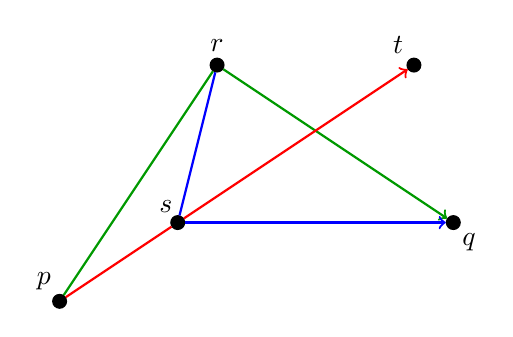
\begin{tikzpicture}
  %\draw[ultra thick, dashed, blue] (5,1) -- (0,0);
  \node[draw, circle, black, fill=black, inner sep=0pt, minimum size=5pt] (p) at (0,0) {};
  \node[] at (-0.2, 0.25) {$p$};
  \node[draw, circle, black, fill=black, inner sep=0pt, minimum size=5pt] (q) at (5,1) {};
  \node[] at (5.2, 0.75) {$q$};
  \node[draw, circle, black, fill=black, inner sep=0pt, minimum size=5pt] (r) at (2,3) {};
  \node[] at (2, 3.25) {$r$};

  \node[draw, circle, black, fill=black, inner sep=0pt, minimum size=5pt] (s) at (1.5, 1) {};
  \node[] at (1.35, 1.2) {$s$};

  \node[draw, circle, black, fill=black, inner sep=0pt, minimum size=5pt] (t) at (4.5, 3) {};
  \node[] at (4.3, 3.25) {$t$};

  \draw[ thick,  green!60!black] (p) -- (r);
  \draw[ thick,  green!60!black, ->] (r) -- (q);

  \draw[ thick,  blue] (r) -- (s);
  \draw[ thick,  blue, ->] (s) -- (q);

  \draw[thick,  red] (p) -- (s);
  \draw[thick,  red, ->] (s) -- (t);
  % \draw[fill=green, opacity=0.5] (a.center) -- (b.center) -- (c.center) -- cycle;
\end{tikzpicture}
\caption{Illustration of triple orientations, where $\sigma(p, r, q) = -1, \sigma(r, s, q) = 1, $ and $\sigma(p, s, t) = 0$.}\label{fig:triple-orientation}
\end{figure}

An example is illustrated in~\Cref{fig:triple-orientation}. We directly use \textsf{mathlib}'s definition of the determinant to define $\sigma$.
% @[pp_dot] abbrev x (p : Point) : ℝ := p 0
% @[pp_dot] abbrev y (p : Point) : ℝ := p 1
\begin{lstlisting}
inductive Orientation : Type where
  | cw -- clockwise :=  -
  | ccw -- counter clockwise := +
  | collinear -- := 0

noncomputable def σ (p q r : Point) : Orientation :=
  let det := Matrix.det !![p.x, q.x, r.x ; p.y, q.y, r.y ; 1, 1, 1]
  if 0 < det then ccw
  else if det < 0 then cw
  else collinear
\end{lstlisting}

% def Orientation.ofReal (r : ℝ) : Orientation :=
%   if 0 < r then ccw
%   else if r < 0 then cw
%   else collinear

Through the $\sigma$ function we can immediately define the notion of \emph{general position} for collections (e.g., finite sets, lists, etc.) of points, simply establishing that $\sigma(p, q, r) \neq 0$ for every three distinct points $p, q, r$ in the collection.
Furthermore, we can start formalizing sets of points that are \emph{equivalent} with respect to their triple orientations, and consequently, properties of pointsets that are fully captured by their triple orientations~(\emph{orientation properties}).
% An illustration is presented in~\Cref{fig:sigma-equiv}.
% \begin{figure}
    \centering
    \begin{subfigure}{0.3\linewidth}
        \centering
        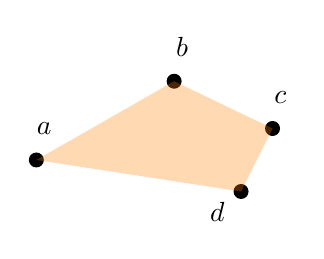
\begin{tikzpicture}
            \node[draw, circle, black, fill=black, inner sep=0pt, minimum size=5pt, label={[xshift=0.1cm, yshift=0.1cm]$a$}] (a) at (0,0) {};
            \node[draw, circle, black, fill=black, inner sep=0pt, minimum size=5pt, label={[xshift=0.1cm, yshift=0.1cm]$b$}] (b) at (1.75,1) {};
            \node[draw, circle, black, fill=black, inner sep=0pt, minimum size=5pt, label={[xshift=0.1cm, yshift=0.1cm]$c$}] (c) at (3,0.4) {};
            \node[draw, circle, black, fill=black, inner sep=0pt, minimum size=5pt, label={[xshift=-0.3cm, yshift=-0.6cm]$d$}] (d) at (2.6,-0.4) {};
            \coordinate (a) at (0,0);
            \coordinate (b) at (1.75,1);
            \coordinate (c) at (3,0.4);
            \coordinate (d) at (2.6,-0.4);
            \fill[orange, opacity=0.3] (a) -- (b) -- (c) -- (d) -- (a) -- cycle;
        \end{tikzpicture}
        \caption{The signature induced by $\sigma$ is $\texttt{-\,-\,-\,-}$.}
    \end{subfigure}
    \begin{subfigure}{0.3\linewidth}
        \centering
        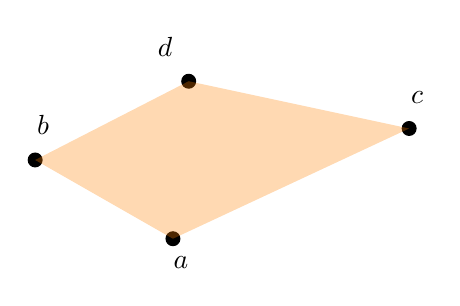
\begin{tikzpicture}
            \node[draw, circle, black, fill=black, inner sep=0pt, minimum size=5pt, label={[xshift=0.1cm, yshift=-0.6cm]$a$}] (a) at (0,0) {};
            \node[draw, circle, black, fill=black, inner sep=0pt, minimum size=5pt, label={[xshift=0.1cm, yshift=0.1cm]$b$}] (b) at (-1.75,1) {};
            \node[draw, circle, black, fill=black, inner sep=0pt, minimum size=5pt, label={[xshift=0.1cm, yshift=0.1cm]$c$}] (c) at (3,1.4) {};
            \node[draw, circle, black, fill=black, inner sep=0pt, minimum size=5pt, label={[xshift=-0.3cm, yshift=0.1cm]$d$}] (d) at (0.2,2) {};
            \coordinate (a) at (0,0);
            \coordinate (b) at (-1.75,1);
            \coordinate (c) at (3,1.4);
            \coordinate (d) at (0.2,2);
            \fill[orange, opacity=0.3] (b) -- (d) -- (c) -- (a) -- (b) -- cycle;
        \end{tikzpicture}
        \caption{The signature induced by $\sigma$ is $\texttt{-\,-\,+\,-}$.}
    \end{subfigure}
    \begin{subfigure}{0.3\linewidth}
        \centering
        
\begin{tikzpicture}
            \node[draw, circle, black, fill=black, inner sep=0pt, minimum size=5pt] (p) at (0,0) {};
        \end{tikzpicture}
    \end{subfigure}
  \caption{Illustration of the notion of $\sigma$-equivalence.}\label{fig:sigma-equiv}
  \end{figure}

\begin{lstlisting}
structure σEquiv (S T : Set Point) where
  f : Point → Point
  bij : Set.BijOn f S T
  parity : Bool -- See Section 4 for a more detailed explanation
  σ_eq : ∀ (p ∈ S) (q ∈ S) (r ∈ S), σ p q r = parity ^^^ σ (f p) (f q) (f r)

def OrientationProperty (P : List Point → Prop) :=
  ∀ {{S T}}, S ≃σ T → (P S ↔ P T) -- `≃σ` is infix notation for `σEquiv`
\end{lstlisting}

To illustrate how these notions will be used, let us consider the property, corresponding to \lstinline|HasConvexEmptyKGon|.
\[
  \pi_k(S) \triangleq \text{\em ``pointset } S \text{ contains an empty convex } k\text{-gon''}.
\]

Based on \lstinline|ConvexEmptyIn.iff_triangles|, we know that $\pi_k(S)$ can be written in terms of triangles that are empty w.r.t $S$. We can define triangle emptiness using $\sigma$, and prove its equivalence to the geoemetric definition.
\begin{lstlisting}
/-- `PtInTriangle a p q r' means that `a' is in the triangle `pqr',
possibly on the boundary. -/
def PtInTriangle (a : Point) (p q r : Point) : Prop :=
  a ∈ convexHull ℝ {p, q, r}

/-- `σPtInTriangle a p q r' means that `a' is in the triangle `pqr' strictly,
i.e., not on the boundary. -/
def σPtInTriangle (a p q r : Point) : Prop :=
  σ p q a = σ p q r ∧
  σ p a r = σ p q r ∧
  σ a q r = σ p q r

theorem σPtInTriangle_iff {a p q r : Point} (gp : InGenPos₄ a p q r) :
  σPtInTriangle a p q r ↔ PtInTriangle a p q r
\end{lstlisting}

% def PtInTriangle (a p q r : Point) : Prop := a ∈ convexHull ℝ {p, q, r}

% def σPtInTriangle (a p q r : Point) : Prop :=
%   σ p q r = σ p a r ∧ σ p a q = σ p r q ∧ σ q a r = σ q p r

% theorem σPtInTriangle_iff {a p q r : Point} (gp : PtFinsetInGenPos {a,p,q,r}) :
%   σPtInTriangle a p q r ↔ PtInTriangle a p q r -- not trivial.

% def HasEmptyTriangle (pts : Set Point) : Prop := ∃ p q r, [p, q, r].Nodup
% ∧ {p,q,r} ⊆ pts ∧ ∀ a ∈ pts, a ∉ ({p, q, r} : Set Point) → ¬PtInTriangle a p q r

% theorem OrientationProperty_HasEmptyTriangle : OrientationProperty HasEmptyTriangle


% Let us now discuss the previous steps. First,~\lstinline|(PtInTriangle a p q r)| presents a \emph{ground-truth}  definition for membership in a triangle, in terms of~\textsf{mathlib}'s \lstinline|ConvexHull| definition,  whereas~\lstinline|(σPtInTriangle a p q r)| is based on orientations.
Heule and Scheucher used the orientation-based definition~\cite{emptyHexagonNumber}, and as it is common in the area, its equivalence to the \emph{ground-truth} mathematical definition was left implicit. This equivalence, proven in~\lstinline|theorem σPtInTriangle_iff| is not trivial to prove, in particular the forward direction requires reasoning about convex combinations and determinants.
Using the previous theorem, we can generalize to $k$-gons as follows.
\begin{lstlisting}
def σHasEmptyKGon (n : Nat) (S : Set Point) : Prop :=
  ∃ s : Finset Point, s.card = n ∧ ↑s ⊆ S ∧
    ∀ (a ∈ s) (b ∈ s) (c ∈ s), a ≠ b → a ≠ c → b ≠ c →
      σIsEmptyTriangleFor a b c S

theorem σHasEmptyKGon_iff_HasEmptyKGon (gp : Point.ListInGenPos pts) :
      σHasEmptyKGon n pts.toFinset ↔ HasEmptyKGon n pts.toFinset
\end{lstlisting}

Then, because \lstinline|σHasEmptyKGon| is ultimately defined in terms of $\sigma$, we can prove
\begin{lstlisting}
lemma OrientationProperty_σHasEmptyKGon : OrientationProperty (σHasEmptyKGon n)
\end{lstlisting}
Which in combination with \lstinline|theorem σHasEmptyKGon_iff_HasEmptyKGon|, provides
\begin{lstlisting}
theorem OrientationProperty_HasEmptyKGon : OrientationProperty (HasEmptyKGon n)
\end{lstlisting}

Let us discuss why the previous theorem is relevant, as it plays an important role in the formalization of Erd\H{o}s-Szekeres-type problems. This boils down to two reasons:
\begin{enumerate}
  \item If we prove that the function $\sigma$ is invariant under a certain transformation of its arguments (e.g., rotations, translations, etc.) then we can directly conclude that any orientation property is invariant under the same transformation. This is a powerful tool for applying manipulations to pointsets that preserve the properties of interest, which will be key for symmetry breaking (see~\Cref{sec:symmetry-breaking}). For a concrete example, when a proof for an Erd\H{o}s-Szekeres-type result starts saying \emph{``we assume without loss of generality that points $p_1, \ldots, p_n$ are sorted from left to right''}, we can immediately formalize that this assumption indeed maintains generality for orientation properties, as sorting a list naturally induces a bijection.
  \item As introduced at the beginning of this section, SAT encodings for Erd\H{o}s-Szekeres-type problems are based on capturing properties like convexity or emptiness in terms of triple orientations, thus reducing a continuous search space to a discrete one. Because we have proved that $\pi_k(S)$ is an orientation property, then the values of $\sigma$ for all triples of points in $S$ is enough information to determine whether $\pi_k(S)$ or not.  Therefore, we have proved that given $n$ points it is enough to analyze the values of $\sigma$ over the points, a discrete space with at most $2^{n^3}$ possibilities, instead of $\left(\mathbb{R}^2\right)^n$. This is the key idea that will allow us to transition from the finitely-verifiable statement \emph{``no set of triple orientations over $n$ points satisfies property $\pi_k$''} to \emph{``no set of $n$ points satisfies property $\pi_k$''}.
\end{enumerate}

\subsection{Properties of orientations}\label{sec:sigma-props}

We now prove that, assuming points will be sorted left to right (which is justified in~\Cref{sec:symmetry-breaking}), then the clauses in~\Cref{eq:signotopeClauses11,eq:signotopeClauses12} are justified.
Consider four points $p, q, r, s$ that are sorted from left to right. If $p, q, r$ are oriented counterclockwise, and $q, r, s$ are oriented counterclockwise as well, then it follows that $p, r, s$ must be oriented counterclockwise too (see~\Cref{fig:orientation-implication}). Different \emph{$\sigma$-implication-properties} of this form are used to reduce the search space in SAT encodings~\cite{emptyHexagonNumber,scheucherTwoDisjoint5holes2020,subercaseaux2023minimizing, szekeres_peters_2006}, as they can be easily added in clausal form:
\begin{align}
  &\left(\neg \orvar_{a, b, c} \lor \neg \orvar_{a, c, d} \lor \orvar_{a, b, d}\right) \land \left(\orvar_{a, b, c} \lor \orvar_{a, c, d} \lor  \neg \orvar_{a, b, d}\right)
\end{align}

We prove these properties of the $\sigma$ function, justifying the addition of~\Cref{eq:signotopeClauses11,eq:signotopeClauses12}, as well as other similar properties that are useful for other proofs, even if not explicitly added to the encoding.
\begin{lstlisting}
theorem σ_prop₁ (h : Sorted₄ p q r s) (gp : InGenPos₄ p q r s) :
    σ p q r = ccw → σ q r s = ccw → σ p r s = ccw

 [...]

theorem σ_prop₃ (h : Sorted₄ p q r s) (gp : InGenPos₄ p q r s) :
    σ p q r = cw → σ q r s = cw → σ p r s = cw
\end{lstlisting}


The proofs of these properties are based on an equivalence between the orientation of a triple of points and the \emph{slopes} of the lines that connect them. Namely, if $p, q, r$  are sorted from left to right, then (i) $\sigma(p,q,r)=1 \iff \textsf{slope}(\overrightarrow{pq}) < \textsf{slope}(\overrightarrow{pr})$  and (ii) $\sigma(p,q,r)=1 \iff \textsf{slope}(\overrightarrow{pr}) < \textsf{slope}(\overrightarrow{qr})$. By proving first these \emph{slope-orientation} equivalences we can then easily prove e.g.,~\lstinline|σ_prop₁|, as illustrated in~\Cref{fig:orientation-implication}.

\begin{figure}
  \centering
  \begin{tikzpicture}
    \newcommand{\localspacing}{4.5}

    \foreach \i in {0, 1, 2} {

      \coordinate (p\i) at ( \i*\localspacing +0.5,0);
      \coordinate (q\i) at ( \i*\localspacing +2.5, 0.75);
      \coordinate (r\i) at ( \i*\localspacing +3.25, 1.5);
      \coordinate (s\i) at ( \i*\localspacing +4.0, 3.25);
    }
    \coordinate (0p) at (13,0);
    \coordinate (0q) at (13, 0.75);
    \coordinate (0r) at (13, 1.5);
    \coordinate (0s) at (13, 3.25);

    \pic [draw, <->,
    angle radius=9mm, angle eccentricity=0.8, fill=blue!20!white,
    "$\text{\tiny{\(\theta_1\)}}$"] {angle = 0p--p0--q0};

    \pic [draw, <->,
    angle radius=7mm, angle eccentricity=0.6, fill=orange!20!white,
    "$\text{\tiny{\(\theta_2\)}}$"] {angle = 0q--q0--r0};


    \pic [draw, <->,
    angle radius=7mm, angle eccentricity=0.6, fill=orange!20!white,
    "$\text{\tiny{\(\theta_2\)}}$"] {angle = 0q--q1--r1};

    \pic [draw, <->,
    angle radius=6mm, angle eccentricity=0.6, fill=yellow!20!white,
    "$\text{\tiny{\(\theta_3\)}}$"] {angle = 0r--r1--s1};


    \pic [draw, <->,
    angle radius=9mm, angle eccentricity=0.8, fill=purple!20!white,
    "$\text{\tiny{\(\theta_4\)}}$"] {angle = 0p--p2--r2};


    \pic [draw, <->,
    angle radius=6mm, angle eccentricity=0.6, fill=yellow!20!white,
    "$\text{\tiny{\(\theta_3\)}}$"] {angle = 0r--r2--s2};



    \foreach \i in {0, 1, 2} {

      \node[draw, circle, black, fill=black, inner sep=0pt, minimum size=5pt] (p\i) at ( \i*\localspacing +0.5,0) {};
      \node[] at ( \i*\localspacing + 0.3, -0.25) {$p$};
      \node[draw, circle, black, fill=black, inner sep=0pt, minimum size=5pt] (q\i) at ( \i*\localspacing +2.5, 0.75) {};
      \node[] at ( \i*\localspacing +2.6, 0.5) {$q$};
      \node[draw, circle, black, fill=black, inner sep=0pt, minimum size=5pt] (r\i) at ( \i*\localspacing +3.25, 1.5) {};
      \node[] at ( \i*\localspacing +3.4, 1.3) {$r$};

      \node[draw, circle, black, fill=black, inner sep=0pt, minimum size=5pt] (s\i) at ( \i*\localspacing +4.0, 3.25) {};
      \node[] at ( \i*\localspacing +4.05, 3) {$s$};
    }

    % \newcommand{\localdx}{0.25}
    % \newcommand{\localdy}{-0.5}
    \draw[thick, green!60!black] (p0) -- (q0);
    \draw[thick, green!60!black, ->] (q0) -- (r0);

    \draw[ thick, green!60!black] (q1) -- (r1);
    \draw[ thick, green!60!black, ->] (r1) -- (s1);

    \draw[ thick, green!60!black] (p2) -- (r2);
    \draw[ thick, green!60!black, ->] (r2) -- (s2);
    % \draw[  dashed, green!60!black] (0 + \localdx, 0 + \localdy) -- (2.5 + \localdx, 0.75 + \localdy);
    % \draw[ dashed, green!60!black, ->] (2.5 + \localdx, 0.75 + \localdy) -- (3.25 + \localdx, 1.5 + \localdy);


    % \draw[  dashed, green!60!black] (2.5  - \localdx, 0.75 - \localdy) -- (3.25 - \localdx, 1.5 - \localdy);
    % \draw[ dashed, green!60!black, ->] (3.25 - \localdx, 1.5 - \localdy) -- (4.25  - \localdx, 3.25 - \localdy);

    % \draw[ thick, dashed, green!60!black] (p) -- (r);
    % \draw[ thick, dashed, green!60!black, ->] (r) -- (s);


    \draw[dashed] (p0) -- (0p);
    \draw[dashed] (q0) -- (0q);
    \draw[dashed] (r0) -- (0r);
    \draw[dashed] (s0) -- (0s);



  \end{tikzpicture}
  \caption{Illustration for $\sigma(p,q,r) = 1 \; \land \; \sigma(q,r,s) = 1 \implies \sigma(p, r, s) = 1$. As we have assumptions $\theta_3 > \theta_2 > \theta_4$  by the forward direction of the \emph{slope-orientation equivalence}, we deduce $\theta_3 > \theta_4$, and then conclude $\sigma(p, r, s) = 1$ by the backward direction of the \emph{slope-orientation equivalence}.  }\label{fig:orientation-implication}
\end{figure}
